\chapter{Introduction} \label{chap:introduction}Economists assert manufacturing to be a wealth-producing sector of an economy, since manufacturing process involve the processes to transform raw materials into finished goods on a large scale. Manufacturing world thrives upon many complex variables. In the recent years, due to innovations in \acs{ICT} the focus of supply and demand are shifting, thus manufacturing industry is experiencing complex supply chains. Customers demanding high levels of individualized products are driving fierce competition in pricing and forcing manufacturers to strive for highest levels of efficiencies. Still manufacturers can develop effective survival strategies amidst all these turbulences \reffig{fig:1.1} if they are able to continuously adapt their organizational structures \cite{WESTKAMP}.

The challenge for adaptive manufacturing is to access all available information when it is needed, where it is needed, and in the form it is most useful to drive optimal actions and responses \refsection{IOT}. Adaptive manufacturing also enables manufacturers to generate and apply data-driven manufacturing intelligence throughout the life-cycle of design, engineering, planning and production.

With the advent of a new wave of technological changes known as Industry 4.0 \refsection{ind4} is already driving a paradigm shift in manufacturing. Manufacturing sector is at the verge of a new industrial revolution which promises all range of opportunities for innovation in terms of smarter industrial processes, new business models and customized products. The new technological wave builds on the concept of interaction between the real and virtual worlds which becomes the core of the manufacturing processes. Both production equipment and manufactured products are now able to gather, process and analyze data of the physical world and interact with each other autonomously.
\begin{figure}[h!]
	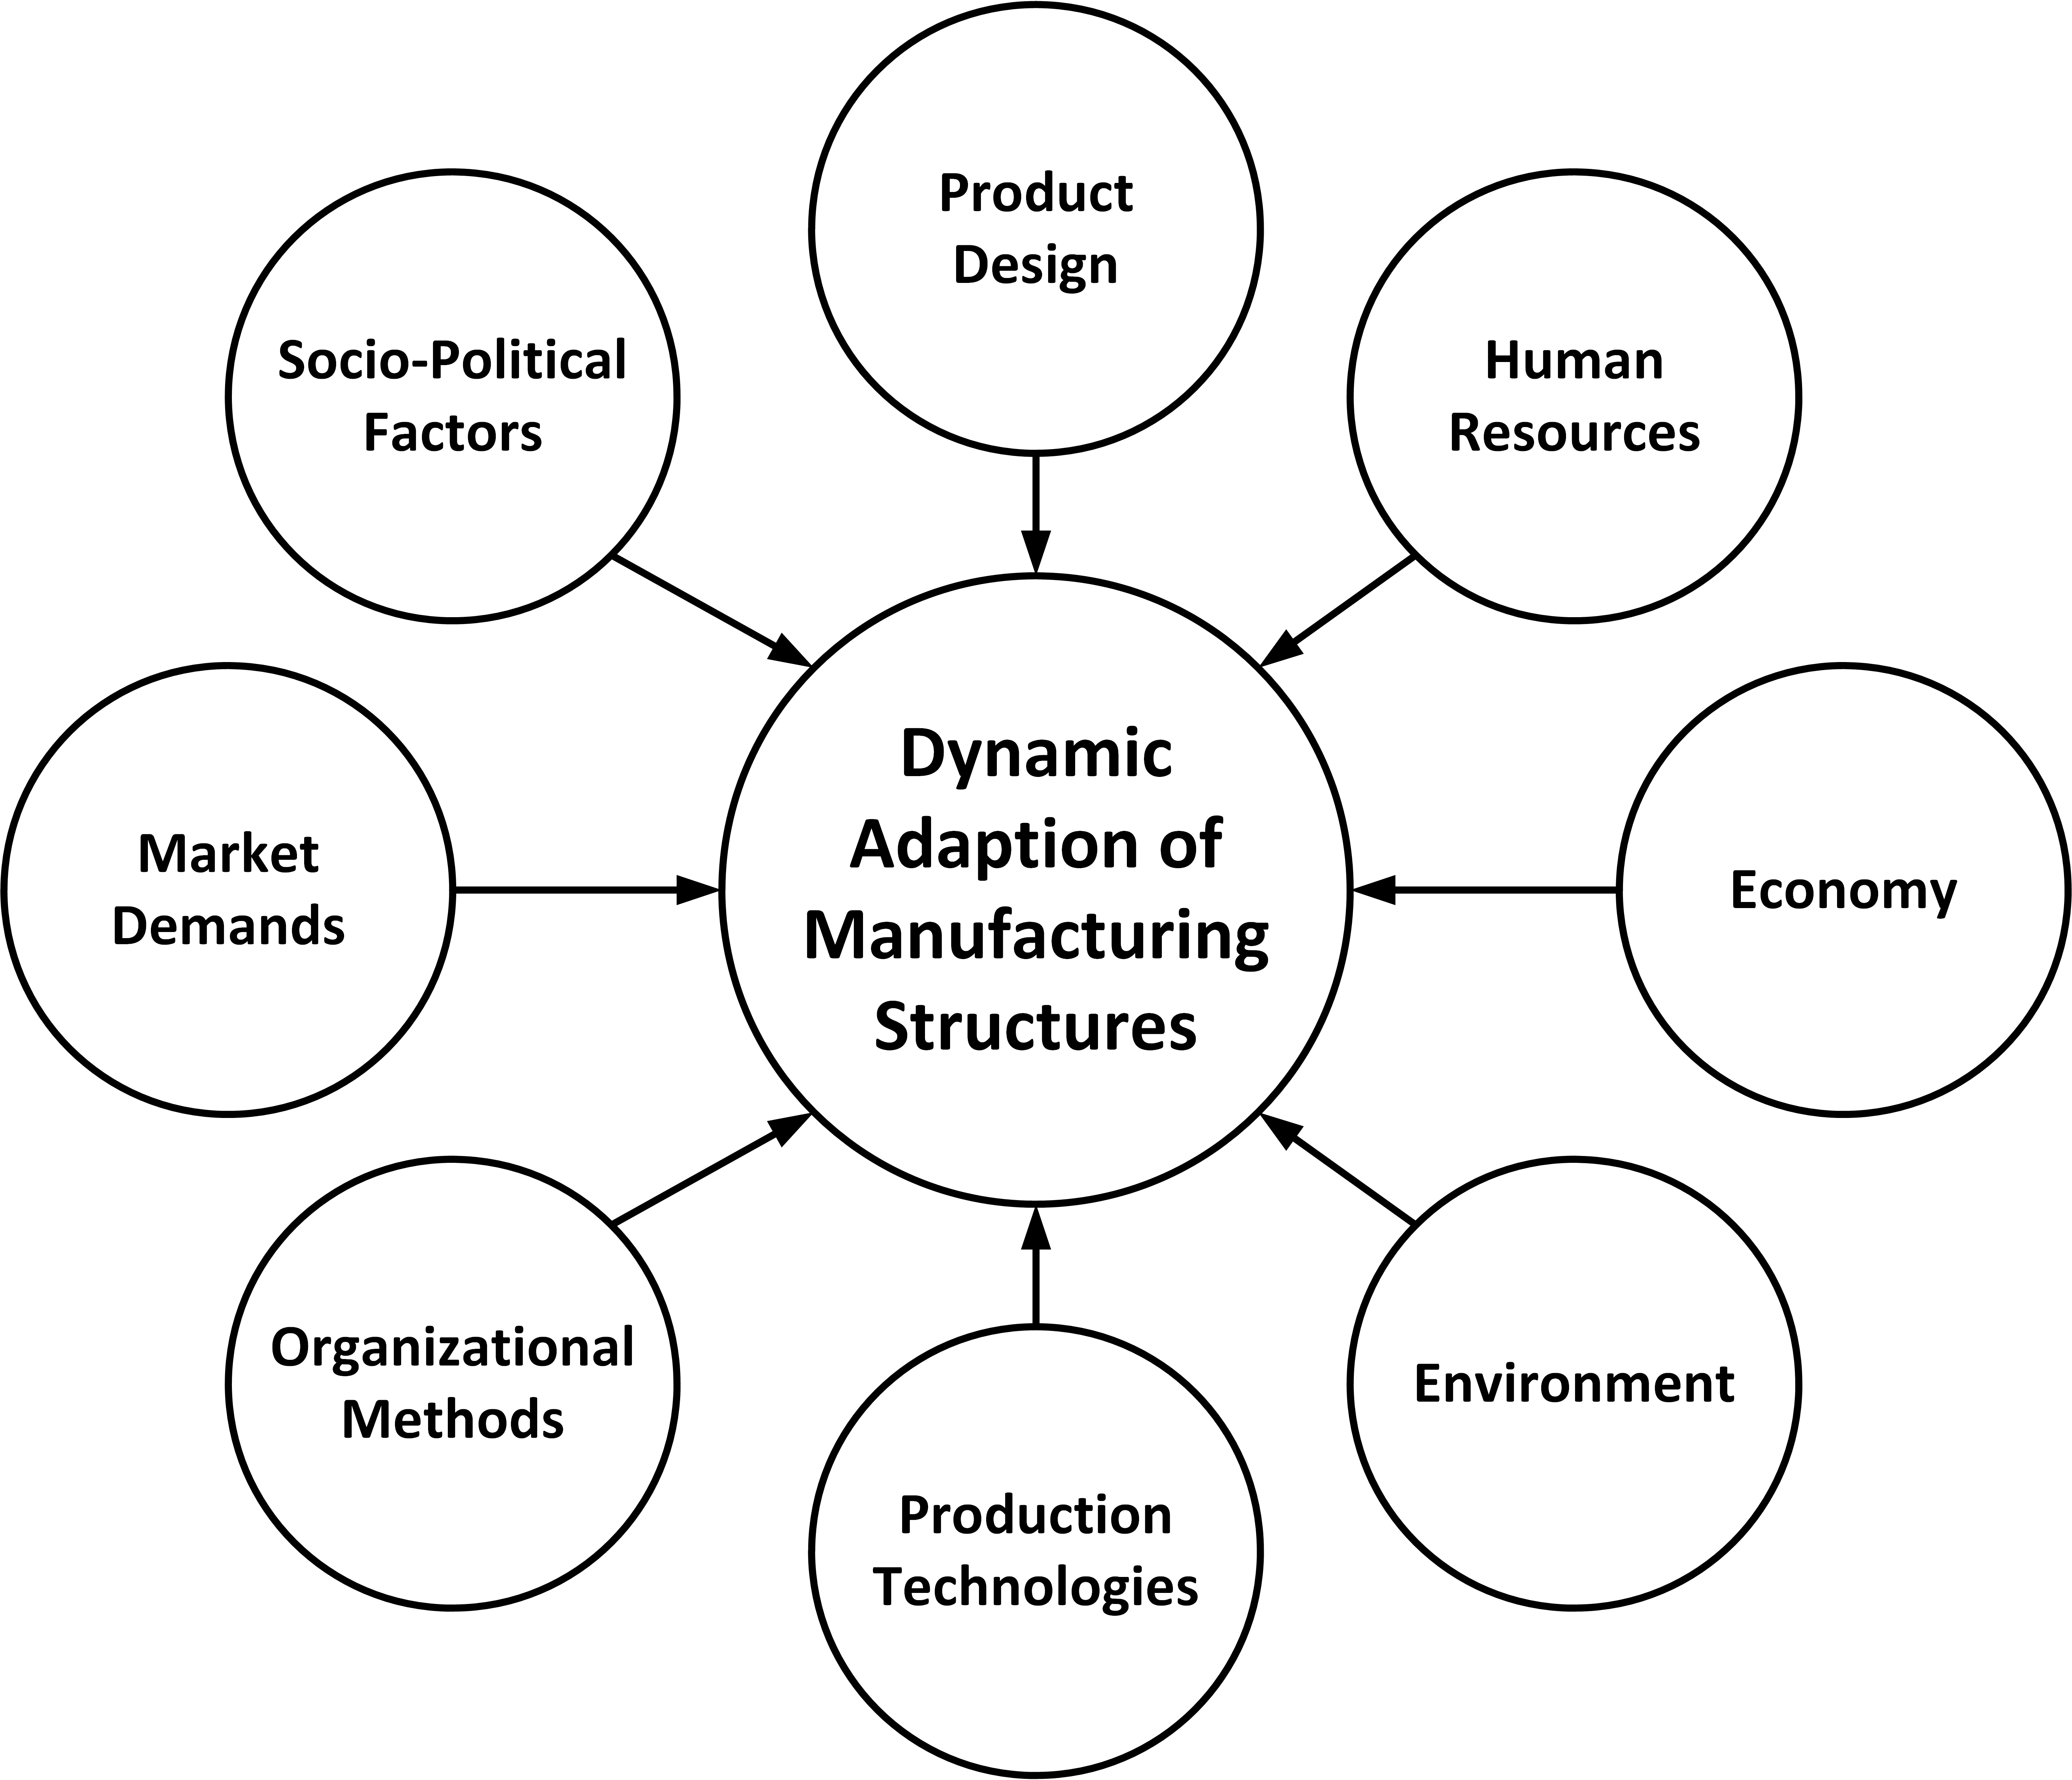
\includegraphics[scale=0.35]{./gfx/addmanustr}
	\centering
	\caption{Adapting the Structures of Manufacturing \cite{WESTKAMP}}
	\label{fig:1.1}
\end{figure}

The primary objectives of production are known as the ‘holy trinity’ of cost,
quality, and time – the sequence varying according to the ‘felt’ importance. Most
important is to point out the right direction of goal achievement – low production
costs, high quality of products, as well as short lead times in production and order
processing. Recently the product variety on offer is added to these production goals. Products produced in series and not positioned within the lowest price segment
can only be distinguished from competition by the ‘long tail’ of innumerable possible
variants or individualized (customized) products - as we refer them \cite{LEANFAC}.
\begin{figure}[h!]
	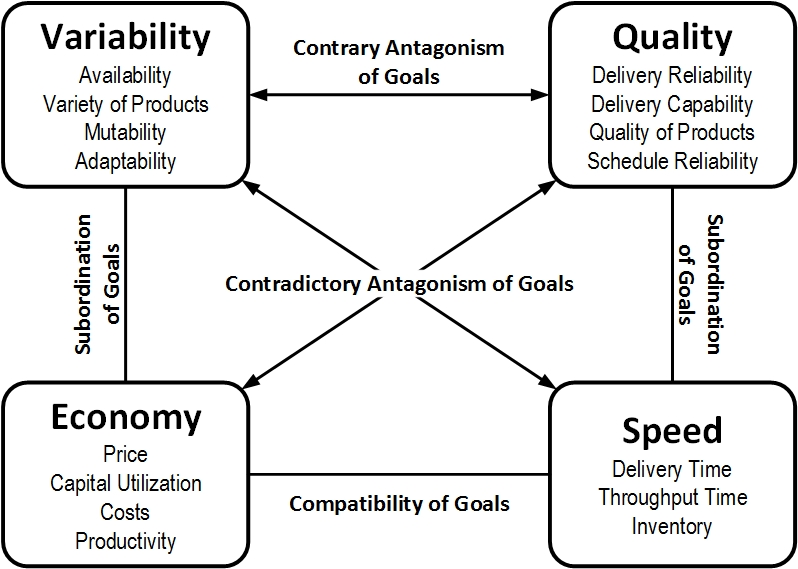
\includegraphics[scale=0.49]{./gfx/4goals}
	\centering
	\caption{Logical Four Square of Conflicting Goals of Production \cite{LEANFAC}}
	\label{fig:1.2}
\end{figure}

Erlach \cite{LEANFAC} explains the relationships between the four goal dimensions and the relevant goal conflicts by the logical square of goals \reffig{fig:1.2}. In sum, the possible relationships between the four goal dimensions can be distinguished into following four types:
\begin{enumerate}
	\item The contradictory antagonism of goals describes the strongest type of conflict where goal achievement for the one goal deteriorates that of the other goal.
	\item The contrary antagonism of goals describes that the attainment of the two goals cannot be improved at the same time, though the fulfillment of the one goal can be improved without negatively affecting the fulfillment of the other goal.
	\item The subordination of goals is possible when attainment of some goals are basically easier to accomplish than others thanks to their lower implementable requirements.
	\item The compatibility of goals exists if the two goals can be better accomplished independently.
\end{enumerate}
Improving the individual goals does not necessarily mean that another goal is affected to the same degree; some goals can actually be improved simultaneously. The objective of production optimization is to counterbalance operation of production and the product range at a specific production site with the four goal dimensions in order to achieve the best level of goal achievement \cite{LEANFAC}.

To increase the efficiency of production process, automation, optimization, and dynamic adaption became the most important requirements in manufacturing sector. Since the dawn of sensors and networking technologies \refsection{IOT} vital information can be gathered before-hand to decide the most suitable and optimized process.  The selection of each execution step may depend on different factors as new technological advancements provide more solution options to the same kind of problems. Manually conducted assembly tasks may provide alternatives to the existing automation methods depending on the current demand, status of the machinery, and occupation of the machinery \cite{TIMURCIRP}. Situations can be observed using smart-systems \refsection{CPS} which enable the application of well-adopted business process modeling and execution  solutions in the context of manufacturing companies and tracking of activity flows in the real world \cite{CONWORKFLOW}.

Production or Manufacturing processes can be modeled using business process modeling languages e.g. the Business Process Execution Language (\acs{BPEL}) \cite{BPELSPEC} or the Business Process Model and Notation (\acs{BPMN}) \cite{OMGSPEC}. After modeling, the process models are deployed on compliant work-flow engines for an automated execution. But these paradigms don not support adaptive and flexible execution of business processes in manufacturing sector. By not considering these adaptations, the manufacturing companies lose their revenue and edge in market by remaining reluctant to structural changes on time \cite{TIMURCIRP,CONWORKFLOW}. The required language constructs have been discussed in later sections \refsection{chap:bpmn}.

\section{Problem Statement}
Manufacturing processes need to be updated regularly to stay competitive in the market was the theme of last section. With the emergence of Internet of Things \refsection{IOT}, the manufacturing processes can be made smarter to leverage the next industrial revolution - Industry 4.0 \refsection{ind4}.

Sungur et al. \cite{TIMURCIRP} presented a novel approach to support \textit{Context-sensitive Adaptive Production Process} in their research work. They extended production processes, which contain a sequence of predefined sets of sub-processes, with \textit{Context-sensitive Execution Steps (\acs{CES})} \refsection{conces}. For each \acs{CES}, context-relevant sub-processes are chosen and desired processes are elected, optimized, deployed and executed \cite{TIMURCIRP}. \acs{CES} approach dictates a way in which processes can possibly adapt themselves to the execution context. In each context, there can be multiple alternatives for the same process goals and the best needs to be selected and executed at runtime \cite{TIMURCIRP}.

In this thesis work, we define a \acs{BPMN} extension which do not change semantics of standard \acs{BPMN} if it's needed at all and adds the necessary details to make manufacturing process models executable. To create this extension, we have- analyzed the properties that make \acs{CES}s unique and also scrutinized important and relevant \acs{BPMN} properties which might be vital during creation of the \acs{CES} extensions. These properties are later on used to derive our requirements from which we create our extension. A summary of the thesis work can be found below \reffig{fig:1.3}.
\begin{figure}[h!]
	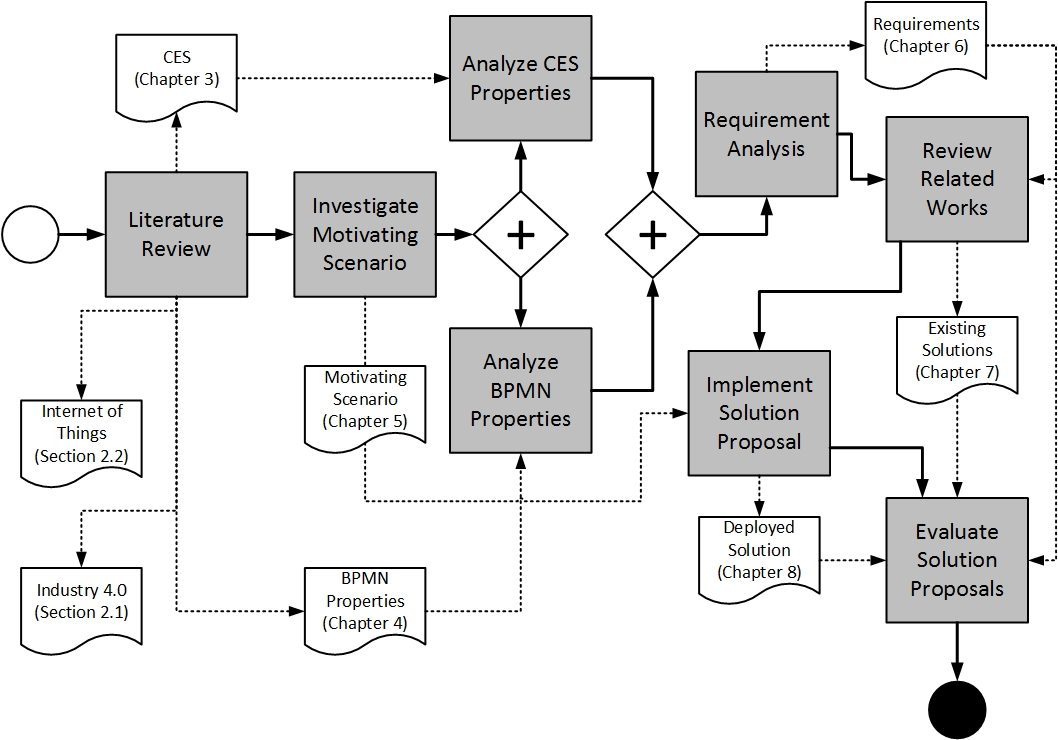
\includegraphics[scale=0.72, angle=90]{./gfx/outline}
	\centering
	\caption{The Thesis Methodology Flow-chart - Inspired from \cite{TIMURTHESIS}}
	\label{fig:1.3}
\end{figure}
\section{Methodology and Outline}
The remaining document is structured in the following way:

The "Literature Review" in this thesis is carried out in three steps as suggested by Levy et al. \cite{LEVYLIT}. We analyzed literature related with Industry 4.0, Internet of Things, \acs{CES}, \acs{BPM} and Efficacies of \acs{BPMN} etc. Main focus during literature review was to understand the current development in Industry 4.0 and it's implications in midst of the innovations in \acs{IoT} technologies. Trends in the \acs{IoT} field has been discussed in detail too. Properties and operational semantics of \acs{CES} are also discussed in the concluding section of the review. After necessary processing corresponding descriptions are touched upon in subsequent section \refsection{chap:fundamentals}.
  
Another part of the literature review is focused upon analyzing properties of \acs{CES}s from standard business processes, and the properties of \acs{BPM} and \acs{BPMN}. This chapter has been added after the initial literature review \refsection{chap:bpmn}. 

For the sake of analysis and apply the conceptual work-flow modeling construct, we have described a motivating scenario depicting a real-world manufacturing scenario which is a mix of manual- and automated task \refsection{chap:motscene}.

In the next chapter, we derive our requirements from the properties that we have found related. By defining our requirements, we conclude the task "Requirement Analysis" in the methodology model \reffig{fig:1.3}. All the relevant properties and requirements for the \acs{CES} have been described in this chapter \refsection{chap:requirements}.

In the next task "Review Related Works", we select and analyze few already existing extensions of \acs{BPMN} or any ongoing work in same direction. We propose our extensions which satisfy the requirements that we have previously defined to make sure that our approach proposed by Sungur et al. \cite{TIMURCIRP} can cater the best to the manufacturing sector \refsection{chap:relatedworks}. 

During the implementation of our conceptual construct, we use the \acs{BPMN} extension methodology and we preserve the semantics of the existing \acs{BPMN} properties. Architecture for the execution of modeled process is touch upon in this chapter \refsection{chap:archimpl}.

In our final task, we evaluate our approach by comparing it with the current state of art or related works already discussed \refsection{chap:relatedworks}. We conclude the task “Evaluate Solution Proposals” by providing this evaluation \refsection{chap:validationevaluation}. 

In the last chapter, we will give a summary and an outlook about our contribution \refsection{chap:outcome}. 

The list containing all the abbreviations or acronyms which are used in this document is added in the appendix \refappendix{acronymlist}.